\documentclass[10pt,twocolumn]{article}

\usepackage[a4paper,margin=1.8cm,columnsep=0.65cm]{geometry}
\usepackage[T1]{fontenc}
\usepackage[utf8]{inputenc}
\usepackage{amsmath}
\usepackage{booktabs}
\usepackage{graphicx}
\usepackage{array}
\usepackage{url}
\usepackage[hidelinks]{hyperref}

\title{\textbf{Residual Reinforcement Learning for Robust Quadrotor Warehouse Navigation:}\\
Paired Isaac Lab Evaluation and Guarded Gazebo/PX4 Transfer}
\author{Berke Tun\c{c}\\AviationSim Project}
\date{August 2026}

\begin{document}
\maketitle

\begin{abstract}
This paper investigates whether residual reinforcement learning (RL), used as a bounded correction to a classical navigation controller, improves quadrotor obstacle-avoidance robustness relative to both the classical controller and a standalone RL policy. Three controllers were evaluated in Isaac Lab under nominal, moderate, and severe perturbations, with 1,024 episodes per controller and condition. The severe evaluation used identical scenario identifiers across controllers. Under severe perturbations, classical control succeeded in 615/1,024 episodes (60.06\%), standalone RL in 834/1,024 (81.45\%), and residual RL in 1,023/1,024 (99.90\%). The residual controller recorded no collisions, compared with 188 for standalone RL. Its Wilson 95\% success interval was 99.45--99.98\%, and exact paired McNemar tests favored it over classical control ($p=3.03\times10^{-123}$) and standalone RL ($p=2.55\times10^{-57}$). On successful severe episodes, residual RL also reduced mean traversal time from 20.87 to 13.17\,s and increased trajectory efficiency from 0.808 to 0.942 relative to classical control. The selected policy was subsequently exported and integrated as a bounded, clearance-shielded, disable-able, fail-closed correction in a ROS~2/Gazebo/PX4 stack. In one paired end-to-end smoke test, both classical and residual-assisted systems navigated and landed successfully; the residual-assisted run was 2.34\,s faster but invoked classical fallback before mission completion. The results provide strong evidence for the research claim inside the Isaac Lab evaluation domain and evidence of guarded transfer feasibility, but not statistical superiority in Gazebo or validation on physical hardware.
\end{abstract}

\section{Introduction}
Autonomous quadrotor navigation in cluttered indoor environments requires a controller to make progress toward a goal while maintaining obstacle clearance, producing smooth commands, and remaining robust to sensing and actuation error. Classical planners provide interpretable geometric behavior, but their fixed assumptions can fail under distribution shift. End-to-end RL can adapt its behavior, yet it may replace useful prior structure and introduce unsafe actions. Residual RL offers a middle ground: a learned policy corrects, rather than replaces, a known controller \cite{johannink2019}.

The AviationSim project studies this design in a warehouse parkour task. A classical flow-field controller supplies the nominal planar velocity. A learned residual observes the goal, velocity, classical proposal, nearby obstacles, and wall clearances, then adds a bounded correction. The comparison also includes an RL policy that directly produces the full navigation command. Training and large-scale evaluation use GPU-parallel Isaac Lab simulation \cite{makoviychuk2021,mittal2025,rudin2022}; deployment evaluation uses ROS~2, Gazebo, and PX4 software-in-the-loop (SITL) \cite{koenig2004,meier2015}.

\section{Motivation, Research Question, and Aim}
The practical motivation is to obtain adaptive obstacle avoidance without discarding a working classical baseline or allowing an unconstrained learned action to control the vehicle. This is especially important when the training simulator abstracts the dynamics that appear in the deployment simulator.

The research question is:

\begin{quote}
Does a bounded residual RL correction improve the robustness, safety, and route quality of quadrotor warehouse navigation relative to classical control and standalone RL, and can the selected policy be transferred into a guarded Gazebo/PX4 follower without preventing end-to-end mission completion?
\end{quote}

The aim is therefore twofold. First, the study tests controller performance at scale under increasing perturbation severity. Second, it evaluates whether the chosen residual policy can be exported and integrated as an optional, bounded, clearance-aware, fail-closed component around the existing follower. The two aims use different standards of evidence: the Isaac Lab claim is supported by 9,216 aggregate evaluation episodes and paired severe-condition tests, whereas the Gazebo transfer result is a diagnostic pair and is interpreted only as feasibility evidence.

\section{Methodology}

\subsection{Task and simulation environment}
The Isaac Lab task uses a $20\times14$\,m room containing 14 staggered, floor-to-ceiling pillars with $0.4\times0.4$\,m footprints. The vehicle starts near $(-8.5,0)$\,m, navigates at a nominal altitude of 1.5\,m, and targets $(8.5,0)$\,m. Goal and collision radii are 0.30 and 0.35\,m, respectively, and the episode limit is 45\,s. Physics advances at 0.01\,s with a decimation of four, yielding a 25\,Hz controller. The vehicle is a simplified velocity-controlled rigid body and obstacle sensing is derived from analytic geometry; consequently, this stage evaluates navigation logic rather than high-fidelity flight dynamics.

The classical controller follows a grid-based flow field with 0.20\,m resolution, 0.60\,m obstacle inflation, and a 1.0\,m/s reference speed. This preserves an interpretable collision-avoidance prior. The deployment planner uses A* search \cite{hart1968} and a lower 0.4\,m/s cruise command in the Gazebo/PX4 system.

\subsection{Controller designs}
Three controller modes were compared:
\begin{enumerate}
    \item \textbf{Classical}: the flow-field proposal is applied without a learned correction.
    \item \textbf{Standalone RL}: the policy directly produces the planar command.
    \item \textbf{Residual RL}: the policy adds a two-dimensional correction to the classical proposal.
\end{enumerate}

The standalone observation has 20 values. Residual control uses 22 values: relative goal position (2), vehicle velocity (2), classical proposal (2), relative positions of the six nearest pillars (12), and four wall clearances. The residual action is scaled to at most 0.75\,m/s per axis, and the combined command is capped at 1.5\,m/s.

\subsection{Learning procedure}
The policy was trained using proximal policy optimization (PPO) \cite{schulman2017}. Actor and critic are separate multilayer perceptrons with two 64-unit ELU hidden layers. The Gaussian policy begins with unit standard deviation. Training used 8,192 parallel environments, 24 steps per environment per iteration, 5,000 iterations, learning rate $5\times10^{-4}$, discount factor 0.99, generalized-advantage parameter 0.95, clipping ratio 0.2, five learning epochs, and four minibatches. This corresponds to
\[
8192\times24\times5000=983{,}040{,}000
\]
simulated transitions for the selected run. The evaluated checkpoint was \path{model_4999.pt} with seed 42.

For distance $d$ to the goal, the potential is
\[
\Phi(d)=1-\tanh(d/3).
\]
The residual reward is
\[
\begin{aligned}
r_t={}&15[\Phi(d_t)-\Phi(d_{t-1})]-0.5\Delta t\\
&-20I_{\mathrm{collision}}+20I_{\mathrm{goal}}\\
&-0.5\lVert a_t^{\mathrm{res}}\rVert\Delta t.
\end{aligned}
\]
The last term discourages unnecessary intervention, while the potential term follows the principle of reward shaping \cite{ng1999}.

\subsection{Robustness evaluation}
Each controller was evaluated for 1,024 episodes under three profiles. Nominal evaluation used the base task. Moderate evaluation introduced spawn jitter of up to $(\pm0.25,\pm0.75)$\,m, actuation gain in $[0.85,1.15]$, wind up to 0.10\,m/s, and observation-noise standard deviation 0.02. Severe evaluation increased these ranges to $(\pm0.50,\pm1.25)$\,m, gain $[0.70,1.30]$, wind 0.20\,m/s, and noise standard deviation 0.05. These perturbations implement a domain-randomization-style robustness test \cite{tobin2017}.

Severe scenarios were formally paired: all controllers received the same 1,024 scenario identifiers, generated with evaluation seed 42, scenario seed 10045, and observation-noise seed 20045. The older moderate artifacts share the intended configuration and run seed but do not record scenario identifiers; moderate results are therefore reported descriptively and are not used for paired inference.

Primary outcomes were success, collision, out-of-bounds termination, and timeout. Route duration, path length, trajectory efficiency, command-variation rate, and clearance were summarized over successful episodes so that stalled or early-collision trajectories did not create misleading route-quality averages. Reliability-adjusted efficiency was defined as success rate multiplied by successful-episode efficiency. Wilson score intervals quantify binomial uncertainty \cite{wilson1927}. Exact two-sided McNemar tests compare severe paired successes using discordant scenario outcomes \cite{mcnemar1947}.

\subsection{Guarded Gazebo/PX4 transfer}
The selected actor was exported to NumPy weights and embedded in the ROS~2 path follower around PX4 SITL and Gazebo. The learned correction is bounded, clearance-shielded, disable-able, and disabled by default. It fails closed to classical control when observations, replans, or policy execution are unsuitable. Classical ArUco-based terminal alignment and landing remain responsible for the final mission phase.

The reported v10 transfer pair used equivalent starts and a 150\,s timeout. Both trials traversed the obstacle course and attempted marker landing. Controller latency, residual inference latency, correction magnitude, shield interventions, navigation outcome, and landing outcome were recorded. Because only one successful pair was collected, no population-level Gazebo significance test is claimed.

\section{Results}

\subsection{Large-scale Isaac Lab comparison}
Table~\ref{tab:isaac} presents the principal results. All controllers achieved 100\% nominal success, but route quality differed: residual RL reduced mean nominal path length from 20.051 to 17.281\,m and increased efficiency from 0.833 to 0.966 relative to classical control. Under moderate perturbations, classical and residual control retained 100\% success, whereas standalone RL succeeded in 919/1,024 episodes (89.75\%) and collided in 105 (10.25\%). Residual RL also produced the highest moderate reliability-adjusted efficiency, 0.945 versus 0.814 for classical and 0.733 for standalone RL.

\begin{table*}[t]
\centering
\caption{Isaac Lab results. Time, path, efficiency, variation, and clearance are means over successful episodes; RA efficiency is reliability-adjusted efficiency. Each row contains 1,024 episodes.}
\label{tab:isaac}
\resizebox{\textwidth}{!}{%
\begin{tabular}{llrrrrrrrr}
\toprule
Profile & Controller & Success & Collision & Time (s) & Path (m) & Efficiency & RA efficiency & Variation (m/s$^2$) & Clearance (m)\\
\midrule
Nominal & Classical & 100.00\% & 0.00\% & 20.050 & 20.051 & 0.8329 & 0.8329 & 8.648 & 0.335\\
Nominal & Standalone RL & 100.00\% & 0.00\% & 13.680 & 20.521 & 0.8138 & 0.8138 & 9.423 & 0.075\\
Nominal & Residual RL & 100.00\% & 0.00\% & 12.000 & 17.281 & 0.9664 & 0.9664 & 1.167 & 0.375\\
\midrule
Moderate & Classical & 100.00\% & 0.00\% & 20.531 & 20.646 & 0.8136 & 0.8136 & 9.241 & 0.367\\
Moderate & Standalone RL & 89.75\% & 10.25\% & 13.629 & 20.461 & 0.8169 & 0.7331 & 9.546 & 0.233\\
Moderate & Residual RL & 100.00\% & 0.00\% & 12.616 & 17.713 & 0.9445 & 0.9445 & 2.633 & 0.410\\
\midrule
Severe & Classical & 60.06\% & 0.00\% & 20.870 & 20.968 & 0.8084 & 0.4855 & 9.380 & 0.375\\
Severe & Standalone RL & 81.45\% & 18.36\% & 14.363 & 20.453 & 0.8183 & 0.6665 & 9.782 & 0.325\\
Severe & Residual RL & 99.90\% & 0.00\% & 13.167 & 17.772 & 0.9423 & 0.9413 & 3.004 & 0.414\\
\bottomrule
\end{tabular}}
\end{table*}

Severe perturbations separated the methods most clearly. Classical control succeeded in 615/1,024 scenarios and timed out in 409. Standalone RL succeeded in 834, collided in 188, and timed out in two. Residual RL succeeded in 1,023, timed out once, and recorded no collision or out-of-bounds termination. Thus residual RL improved success by 39.84 percentage points over classical control and 18.46 points over standalone RL.

The severe Wilson 95\% success intervals were 57.03--63.02\% for classical control, 78.95--83.71\% for standalone RL, and 99.45--99.98\% for residual RL. In the paired comparison with classical control, residual RL won all 408 discordant scenarios and lost none ($p=3.03\times10^{-123}$). Against standalone RL it won all 189 discordant scenarios and lost none ($p=2.55\times10^{-57}$). Standalone RL beat classical control in 322 discordant scenarios and lost 103 ($p=2.49\times10^{-27}$), but its gain in completion came with an 18.36\% collision rate.

Among successful severe episodes, residual RL was 7.703\,s (36.9\%) faster than classical control, shortened the mean path by 3.196\,m (15.2\%), raised efficiency by 0.134, and reduced command-variation rate from 9.380 to 3.004\,m/s$^2$. Its mean minimum clearance was also 0.039\,m greater. These results show that the success advantage was not obtained through more erratic commands or systematically smaller clearance.

\begin{figure*}[t]
\centering
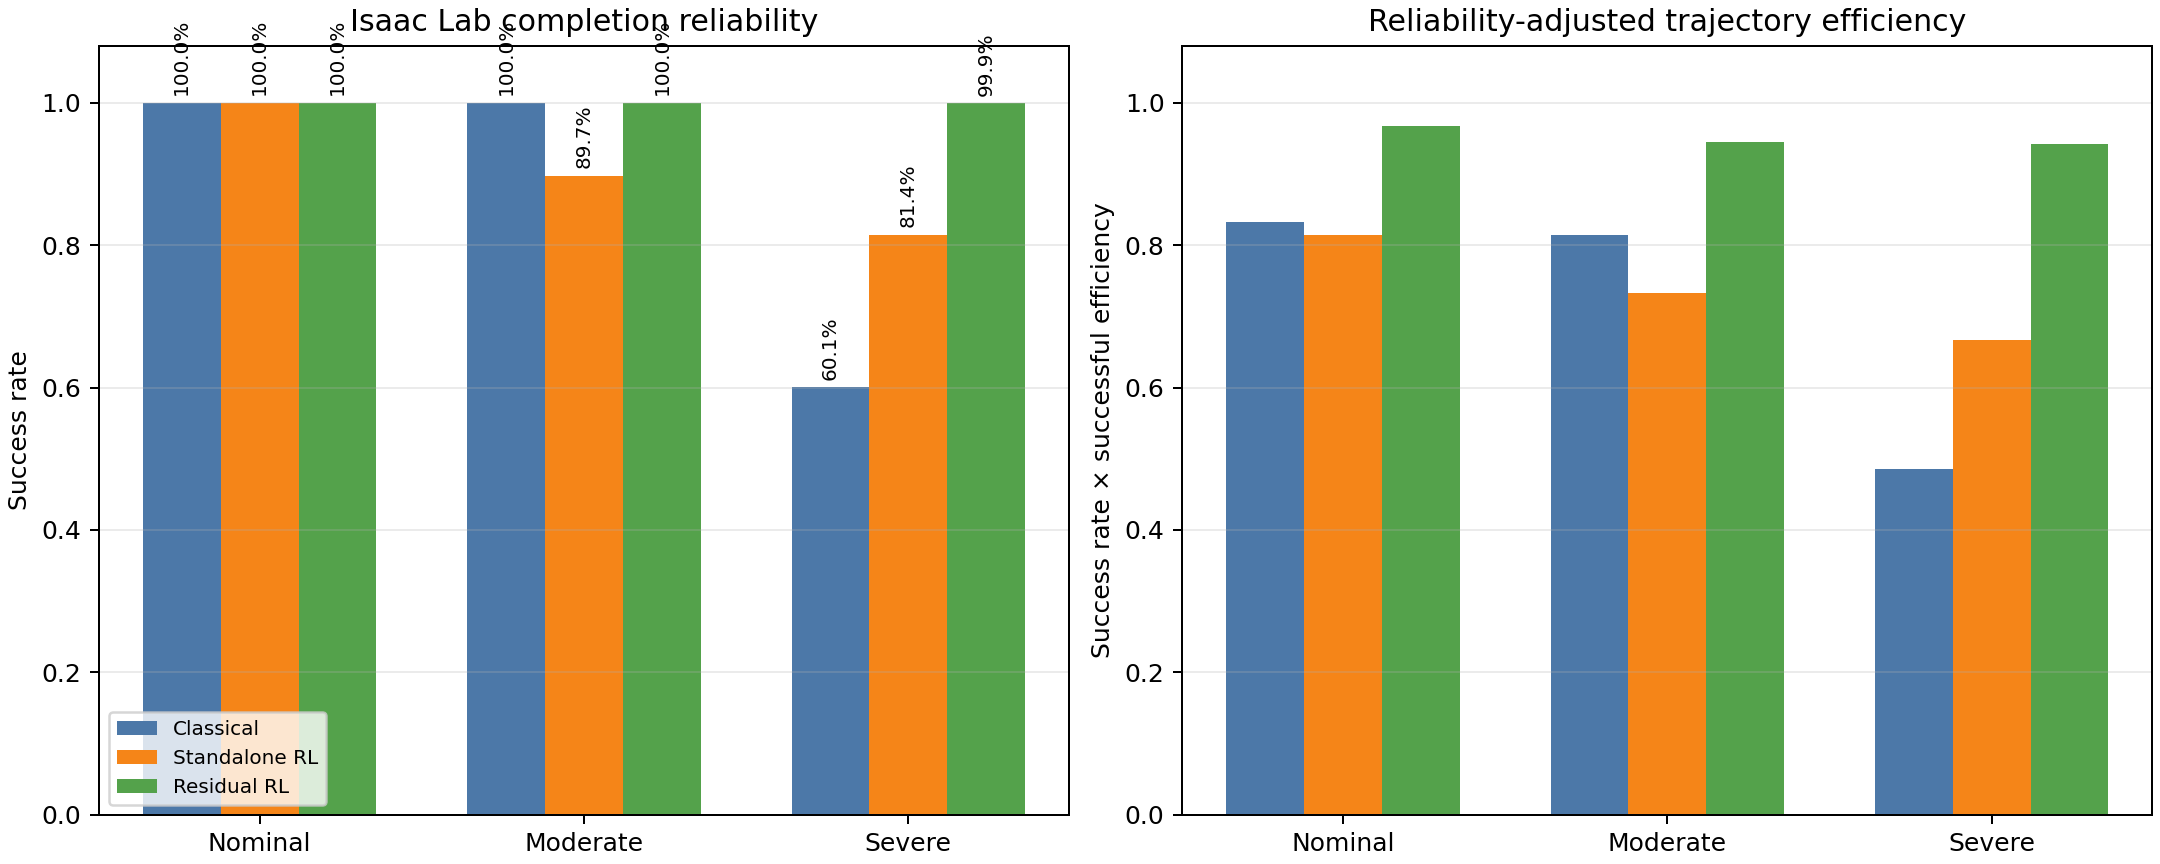
\includegraphics[width=0.96\textwidth]{plots/isaac_controller_comparison.png}
\caption{Controller comparison across nominal, moderate, and severe Isaac Lab evaluations.}
\label{fig:isaac}
\end{figure*}

\subsection{Initialization ablation}
An identity warm start first achieved an open-loop imitation mean-squared error of $4.65\times10^{-5}$, but the small remaining action error produced a mean 0.193\,m/s closed-loop correction and 0/1,024 successes. Exact zero projection restored the classical controller and 100\% success, demonstrating that near-zero supervised error is not equivalent to closed-loop identity.

At equal PPO budgets, random initialization learned faster than the identity initialization. After 50 iterations, random initialization achieved 14.560\,s mean successful duration, 0.9157 efficiency, and 0.298\,m/s mean residual magnitude, compared with 19.215\,s, 0.8480, and 0.046\,m/s for identity initialization. At 100 iterations, the values were 12.480\,s, 0.9543, and 0.526\,m/s for random initialization versus 17.663\,s, 0.8674, and 0.109\,m/s for identity initialization. The 100-iteration fine-tune used 19,660,800 transitions and took 52.67\,s. The optional checkpoint-under-perturbation study was not performed, so this ablation concerns nominal training behavior rather than robustness rankings.

\subsection{Gazebo/PX4 transfer}
Both v10 smoke trials completed navigation and precision landing (Table~\ref{tab:gazebo}). Classical control finished in 76.52\,s over 18.198\,m. Residual-assisted control finished in 74.18\,s over 17.988\,m: 2.34\,s (3.1\%) faster and 0.210\,m (1.2\%) shorter in this pair. Final goal distance improved by 0.008\,m, while minimum clearance decreased from 0.711 to 0.682\,m. The latter remained 0.332\,m beyond the 0.35\,m collision radius.

\begin{table}[t]
\centering
\caption{Paired v10 Gazebo/PX4 diagnostic trial.}
\label{tab:gazebo}
\resizebox{\columnwidth}{!}{%
\begin{tabular}{lrr}
\toprule
Metric & Classical & Residual-assisted\\
\midrule
Navigation & Success & Success\\
Landing & Success & Success\\
Duration (s) & 76.52 & 74.18\\
Path length (m) & 18.198 & 17.988\\
Final distance (m) & 0.265 & 0.257\\
Minimum clearance (m) & 0.711 & 0.682\\
Control latency (ms) & 0.035 & 0.294\\
\bottomrule
\end{tabular}}
\end{table}

The residual applied a mean correction of 0.095\,m/s and triggered 189 shield interventions. Inference covered 679 of 1,462 controller samples (46.4\%). An empty replan then caused the designed permanent fallback, so the residual was inactive at mission completion and classical marker guidance performed landing. Mean controller latency increased by 0.259\,ms to 0.294\,ms, still far below the 50\,ms command period. Figure~\ref{fig:gazebo} summarizes the pair.

\begin{figure}[t]
\centering
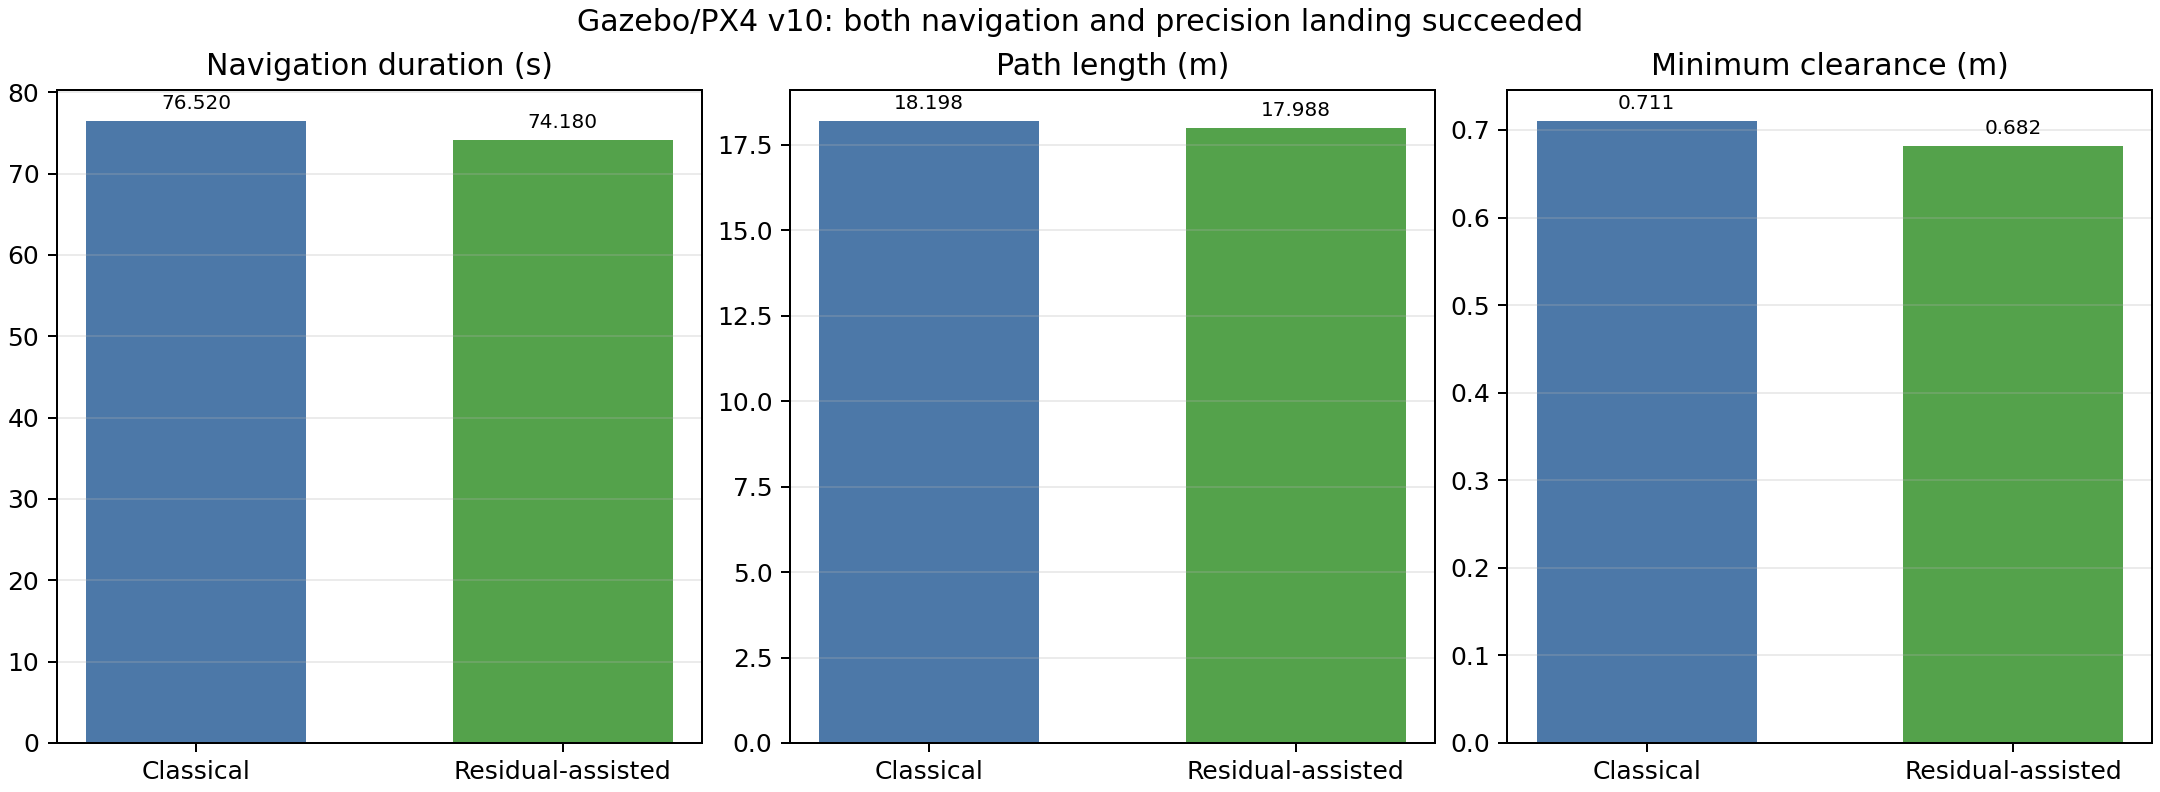
\includegraphics[width=\columnwidth]{plots/gazebo_v10_pair.png}
\caption{Classical and residual-assisted outcomes in the v10 Gazebo/PX4 pair.}
\label{fig:gazebo}
\end{figure}

Earlier transfer attempts are important negative evidence. A v3 residual run timed out after 150.04\,s at 7.569\,m from the goal; an experimental v4 recovery collided after 53.44\,s at 0.342\,m clearance; and v5 fail-closed control avoided collision but timed out at 150.00\,s. A separate command-transport defect was then identified: velocity commands accumulated in an unbounded first-in-first-out queue faster than MAVSDK consumed them. Replacing queued velocity events with latest-value consumption removed stale-command accumulation before the successful v10 pair.

\section{Discussion}
The Isaac Lab evidence answers the first part of the research question affirmatively for the tested domain. Under the strongest perturbations, residual RL nearly eliminated failures while simultaneously improving successful-route efficiency, smoothness, and average clearance. The paired outcome pattern is particularly strong: residual RL never lost a severe scenario that either comparator won, while winning 408 cases over classical control and 189 over standalone RL. The standalone policy improved completion relative to classical control but converted many classical timeouts into collisions, illustrating why success rate alone is insufficient for safety-oriented comparison.

The likely benefit of the residual structure is that it preserves the global directional prior of the classical field while learning locally useful corrections. The residual penalty and action bounds constrain needless deviations, and the classical proposal is explicitly available in the observation. The result is not merely a compromise between the two baselines: residual RL achieved both higher severe success and lower command variation than either.

The second part of the research question has a narrower answer. The exported policy can participate in an end-to-end Gazebo/PX4 mission when surrounded by bounds, a clearance shield, and fail-closed fallback. The v10 pair demonstrates functional integration and acceptable computational latency. It does not demonstrate uninterrupted direct policy transfer, because the residual ran for 46.4\% of controller samples and classical control completed the mission after fallback. Nor does a single pair establish a reliable Gazebo performance advantage.

\section{Limitations and Threats to Validity}
The Isaac vehicle uses simplified velocity dynamics and analytic obstacle observations, so its results should not be interpreted as full aerodynamic validation. The evaluation reuses the same warehouse structure and controller interfaces used during development, although perturbation draws are held out. Severe trials are paired and support paired tests; legacy moderate artifacts lack recorded scenario identifiers and support descriptive comparisons only.

The Gazebo evidence contains one successful v10 pair, with small differences that may be caused by start-state and simulation variation. Earlier failures also show that planner state, policy state, and transport semantics can dominate transfer behavior. No physical-aircraft experiment has been conducted. Finally, the residual checkpoint underwent extensive development selection, so claims should remain tied to the specified task, profiles, and seeds until replicated across maps, seeds, policy checkpoints, and hardware.

\section{Conclusion}
A bounded residual PPO policy provided the strongest tested controller in Isaac Lab. Across 1,024 severe paired scenarios it achieved 99.90\% success with zero collisions, compared with 60.06\% for classical control and 81.45\% with 18.36\% collisions for standalone RL. It also cut successful traversal time by 36.9\% and increased efficiency from 0.808 to 0.942 relative to classical control. Exact paired tests and confidence intervals support this conclusion within the simulation domain.

The exported controller also completed one Gazebo/PX4 navigation-and-landing trial as part of a guarded hybrid, finishing 3.1\% faster than the paired classical trial. Because it fell back to classical control and because $n=1$ paired mission is not a statistical benchmark, the correct conclusion is guarded transfer feasibility rather than proven deployment superiority. The next experimental step is a pre-registered, repeated paired Gazebo campaign across scenario seeds, followed by hardware-in-the-loop and carefully bounded flight tests.

\section*{Reproducibility}
Raw summaries, episode-level CSV files, generated comparisons, and plotting inputs are stored under \path{oa_rl/results/evaluations} and \path{oa_rl/results/gazebo_transfer}. The principal severe report is \path{severe_robustness_comparison.md}; the deployment pair is \path{gazebo_v10_comparison.md}. Software recorded for the severe evaluation included Python 3.11.15, PyTorch 2.7.0+cu128, RSL-RL 5.0.1, Isaac Lab 0.54.4, and Isaac Lab RL 0.5.2.

\begin{thebibliography}{99}
\bibitem{hart1968}
P. E. Hart, N. J. Nilsson, and B. Raphael,
"A Formal Basis for the Heuristic Determination of Minimum Cost Paths,"
\emph{IEEE Transactions on Systems Science and Cybernetics}, vol. 4, no. 2,
pp. 100--107, 1968. doi: 10.1109/TSSC.1968.300136.

\bibitem{schulman2017}
J. Schulman, F. Wolski, P. Dhariwal, A. Radford, and O. Klimov,
"Proximal Policy Optimization Algorithms,"
\emph{arXiv preprint arXiv:1707.06347}, 2017.

\bibitem{johannink2019}
T. Johannink, S. Bahl, A. Nair, J. Luo, A. Kumar, M. Loskyll,
J. A. Ojea, E. Solowjow, and S. Levine,
"Residual Reinforcement Learning for Robot Control,"
in \emph{Proc. IEEE International Conference on Robotics and Automation},
pp. 6023--6029, 2019. doi: 10.1109/ICRA.2019.8794127.

\bibitem{makoviychuk2021}
V. Makoviychuk et al.,
"Isaac Gym: High Performance GPU-Based Physics Simulation for Robot Learning,"
\emph{arXiv preprint arXiv:2108.10470}, 2021.

\bibitem{rudin2022}
N. Rudin, D. Hoeller, P. Reist, and M. Hutter,
"Learning to Walk in Minutes Using Massively Parallel Deep Reinforcement Learning,"
in \emph{Proceedings of the 5th Conference on Robot Learning},
PMLR, vol. 164, pp. 91--100, 2022.

\bibitem{mittal2025}
M. Mittal et al.,
"Isaac Lab: A GPU-Accelerated Simulation Framework for Multi-Modal Robot Learning,"
\emph{arXiv preprint arXiv:2511.04831}, 2025.

\bibitem{meier2015}
L. Meier, D. Honegger, and M. Pollefeys,
"PX4: A Node-Based Multithreaded Open Source Robotics Framework for Deeply Embedded Platforms,"
in \emph{Proc. IEEE International Conference on Robotics and Automation},
pp. 6235--6240, 2015. doi: 10.1109/ICRA.2015.7140074.

\bibitem{koenig2004}
N. Koenig and A. Howard,
"Design and Use Paradigms for Gazebo, an Open-Source Multi-Robot Simulator,"
in \emph{Proc. IEEE/RSJ International Conference on Intelligent Robots and Systems},
pp. 2149--2154, 2004. doi: 10.1109/IROS.2004.1389727.

\bibitem{tobin2017}
J. Tobin et al.,
"Domain Randomization for Transferring Deep Neural Networks from Simulation to the Real World,"
in \emph{Proc. IEEE/RSJ International Conference on Intelligent Robots and Systems},
2017. doi: 10.1109/IROS.2017.8202133.

\bibitem{ng1999}
A. Y. Ng, D. Harada, and S. Russell,
"Policy Invariance Under Reward Transformations: Theory and Application to Reward Shaping,"
in \emph{Proc. 16th International Conference on Machine Learning},
pp. 278--287, 1999.

\bibitem{wilson1927}
E. B. Wilson,
"Probable Inference, the Law of Succession, and Statistical Inference,"
\emph{Journal of the American Statistical Association}, vol. 22, no. 158,
pp. 209--212, 1927. doi: 10.1080/01621459.1927.10502953.

\bibitem{mcnemar1947}
Q. McNemar,
"Note on the Sampling Error of the Difference Between Correlated Proportions or Percentages,"
\emph{Psychometrika}, vol. 12, pp. 153--157, 1947.
doi: 10.1007/BF02295996.
\end{thebibliography}

\end{document}
